\section{开发环境}\label{sec:DevelopmentEnvironment}

在本节(\cref{sec:DevelopmentEnvironment})中,

\subsection{开发环境概述}

本项目的开发环境如下:

\begin{enumerate}
    \item 开发环境
          \begin{enumerate}
              \item Windows 11 家庭中文版 23H2
              \item Windows Subsystem for Linux (WSL) 2.2.4.0
              \item Ubuntu 22.04.3 LTS
              \item QEMU 模拟机(qemu-system-i386)6.2.0
          \end{enumerate}
    \item 开发软件
          \begin{enumerate}
              \item JetBrains RustRover 2024.1.7
          \end{enumerate}
    \item 开发语言
          \begin{enumerate}
              \item Rust 语言(Rustup:1.27.1,Rustc:1.82.0-nightly,Cargo:1.82.0-nightly)
          \end{enumerate}
\end{enumerate}

\subsubsection{Windows 11}

使用Windows系统来开发操作系统内核,尽管可能不如Linux环境那样常见,但仍然有其独特的优势和便利性。以下是使用Windows系统开发操作系统内核的几个主要优势:

\begin{enumerate}
    \item \textbf{熟悉的开发环境}:对于习惯使用Windows的开发者来说,继续在这个环境下工作可以减少学习新工具和操作系统的时间,使他们能够更专注于开发工作本身。Windows的用户界面、文件系统管理、任务管理等都是开发者熟悉的。
    \item \textbf{强大的开发工具}:Windows支持多种强大的开发环境,如Visual Studio Code。这些IDE提供了先进的代码编辑、项目管理、版本控制和调试工具。
    \item \textbf{使用WSL提升开发效率}:通过集成了WSL(Windows Subsystem for Linux),Windows环境可以无缝地运行Linux工具和软件,结合了Linux的命令行工具和Windows的图形界面优势。这允许开发者在不离开Windows的情况下使用Linux环境,例如使用GCC、Make、GDB等工具进行内核开发。
    \item \textbf{文档和社区资源}:Windows拥有庞大的开发者社区和丰富的文档资源,对于解决开发中的问题和学习新技术都极为有用。
\end{enumerate}

总体而言,虽然Linux通常是内核开发的首选环境,但Windows提供的工具、支持和兼容性使其成为许多情况下一个可行且有效的选择,尤其是结合了WSL后,Windows在操作系统内核开发方面的适用性大大提高。

\subsubsection{Windows Subsystem for Linux (WSL)}

使用 Windows Subsystem for Linux (WSL) 在开发操作系统内核时具有一系列优势,特别是对于习惯使用Windows环境的开发者来说。这些优势包括:

\begin{enumerate}
    \item \textbf{集成Windows和Linux环境}:WSL允许开发者在Windows系统上运行Linux环境,无需重启进入另一个操作系统或使用虚拟机。这意味着可以利用Windows的图形界面和生产力工具(如VSCode),同时执行Linux命令行工具和应用。
    \item \textbf{简化开发流程}:对于需要同时访问Windows和Linux工具的开发任务,WSL提供了极大的便利。开发者可以在相同的文件系统中访问项目文件,使用Windows编辑器编辑代码,然后在Linux环境中编译和测试,无需文件转移或复制。
    \item \textbf{资源占用更少}:与传统的虚拟机相比,WSL提供了更轻量级的解决方案。它直接在Windows内核上运行,减少了资源占用,启动和运行速度更快,对系统性能的影响也更小。
    \item \textbf{方便的环境管理}:WSL允许开发者安装多个Linux发行版,可以在不同的项目或任务之间切换不同的环境。例如,可以在一个发行版上进行开发工作,而在另一个发行版上进行测试。
    \item \textbf{直接访问硬件和系统调用}:WSL使用真实的Linux内核,这使得它在处理系统调用和操作硬件时表现得更接近传统Linux系统。这对于需要进行底层系统开发的项目尤其重要,因为它允许开发者在接近生产环境的条件下测试和开发。
    \item \textbf{持续集成和交叉编译支持}:使用WSL,开发者可以在同一机器上进行交叉编译,为不同的平台构建应用程序,包括Linux、Windows和其他操作系统。这种能力对于开发涉及多平台支持的内核或应用程序非常有用。
    \item \textbf{社区和官方支持}:Microsoft对WSL的持续更新和支持确保了其与现代硬件和软件技术的兼容性。此外,广泛的开发者社区也提供了大量的教程、工具和第三方应用支持,这对于解决开发中的问题非常有帮助。
\end{enumerate}

WSL是为那些想要在Windows系统上利用Linux开发工具的开发者提供了一种非常实用的解决方案,它结合了两个系统的优点,提高了开发效率和灵活性。

\subsubsection{Ubuntu 22.04 LTS}

使用Ubuntu作为开发环境,尤其是在开发操作系统内核这类底层项目时,有几个显著的优势:

\begin{enumerate}
    \item \textbf{稳定性和长期支持}:Ubuntu 22.04 LTS(Long Term Support,长期支持)版本提供了长达五年的安全更新和维护。这意味着开发者可以在一个稳定且长期受支持的平台上工作,无需担心频繁更换操作系统或缺乏安全更新。
    \item \textbf{与生产环境一致}:在Ubuntu上开发可以确保软件在生产环境中运行时表现得更加可靠和高效,因为开发和生产环境可以保持高度一致。
    \item \textbf{广泛的社区支持和资源}:Ubuntu拥有庞大的用户和开发者社区,这意味着大量的文档、论坛和支持资源可供查阅。这对于解决开发中遇到的问题非常有帮助。
    \item \textbf{开源工具和库的兼容性}:Ubuntu提供了丰富的开源开发工具和库。对于操作系统开发而言,这些工具(如GCC、Make、GDB)都是不可或缺的,而且通常在Linux系统上的兼容性和性能都非常好。
    \item \textbf{适合底层开发}:Linux系统提供了丰富的底层系统调用和接口,这对于内核开发是非常重要的。开发者可以直接与硬件和底层系统资源交互,更方便地实现和测试内核级功能。
    \item \textbf{环境一致性和隔离性}:使用容器和虚拟化技术(如Docker和QEMU),可以在Ubuntu上轻松创建和管理隔离的开发环境。这对于测试不同的配置和开发环境至关重要。
\end{enumerate}

总之,选择Ubuntu作为开发环境,可以为操作系统内核的开发提供一个稳定、高效、兼容性好的基础,同时也利于将来在类似环境中部署和运行。

\subsubsection{QEMU 模拟机(qemu-system-i386)}

QEMU是一个功能强大的开源机器模拟器和虚拟化解决方案,对于操作系统内核的开发尤为重要。以下是使用QEMU的一些主要优势:

\begin{enumerate}
    \item \textbf{多平台支持}:QEMU能够模拟多种处理器架构,包括x86、ARM、PowerPC、SPARC、和MIPS等。这意味着开发者可以在一个平台上开发和测试为其他平台设计的内核和应用程序,非常适合交叉平台开发。
    \item \textbf{环境隔离}:使用QEMU进行开发可以确保测试环境与主机操作系统隔离。这种隔离可以防止潜在的软件错误影响到主机系统,特别是在开发涉及底层硬件交互的系统软件时。
    \item \textbf{无需实际硬件}:QEMU允许开发者在没有物理目标硬件的情况下进行开发和测试。这不仅降低了成本,还可以在硬件到达前开始开发工作,加速开发周期。
    \item \textbf{调试支持}:QEMU与各种调试工具(如GDB)集成,可以进行详细的步进执行和调试。这对于操作系统内核开发尤为重要,因为它允许开发者在内核运行时进行观察和修改。
    \item \textbf{快照和即时状态保存}:QEMU支持保存和恢复虚拟机的状态(称为快照)。这使得开发者可以快速回滚到一个已知的良好状态,并从那里重新开始测试,极大地提高了测试的效率。
    \item \textbf{网络模拟}:QEMU还能模拟网络环境,允许开发者测试内核的网络功能,如协议栈和驱动程序,而无需实际的网络硬件。
    \item \textbf{性能和资源利用}:虽然QEMU为功能丰富性提供了强大的支持,但它在性能上的优化也非常有效。QEMU的用户模式模拟可以运行应用程序和驱动程序,而不必模拟整个操作系统,从而减少资源消耗。
    \item \textbf{版本更新和社区支持}:QEMU持续更新和改进,提供了最新的功能和改进,确保开发者可以利用最新的技术进行开发。同时,QEMU的广泛用户和开发者社区提供了丰富的文档、工具和支持。
\end{enumerate}

总体来说,QEMU提供了一个强大、灵活、成本效益高的平台,用于开发、测试和调试操作系统内核和其他系统级软件,特别是在多架构和虚拟化环境中。这使得它成为操作系统开发者的重要工具。

\subsubsection{JetBrains RustRover}

JetBrains的RustRover是一款专门为Rust语言设计的集成开发环境(IDE),其提供了许多功能来支持Rust开发,特别是在开发操作系统内核这类复杂项目时。在使用RustRover开发操作系统内核时,具有如下优势:

\begin{enumerate}
    \item \textbf{代码编辑与分析}:RustRover提供了强大的代码编辑器,支持代码高亮、自动格式化、智能补全等功能,能够极大地提高代码编写的效率。它具备深度的代码分析功能,可以帮助开发者快速定位到潜在的代码问题,比如生命周期错误、类型不匹配等常见于Rust开发中的问题。
    \item \textbf{高级调试工具}:RustRover集成了强大的调试器,支持条件断点、表达式求值、变量观察等功能,这对于操作系统内核的调试至关重要。支持对内存布局、堆栈跟踪等低级特性进行检查,这对于底层系统编程尤其有用。
    \item \textbf{跨平台支持和远程开发}:RustRover支持跨平台开发,可以在Windows、Linux或macOS上进行Rust开发。它还支持远程开发功能,允许开发者在远程服务器上直接编写代码、编译和调试,这对于操作系统开发尤其重要,因为操作系统常常需要在特定硬件或仿真环境(如QEMU)中运行和测试。
    \item \textbf{版本控制集成}:RustRover提供了与Git等版本控制系统的无缝集成,这使得管理大型项目的源代码变得更为方便。
    \item \textbf{项目和构建管理}:该IDE提供了对Cargo的完整支持,包括依赖管理、构建配置和测试,并可以直接从IDE中运行构建脚本和测试,极大地简化了构建过程。
    \item \textbf{社区和插件}:JetBrains拥有活跃的开发者社区,可以轻松找到大量有用的插件和资源,以扩展IDE的功能并适应特定开发需求。
\end{enumerate}

总的来说,RustRover为Rust操作系统内核开发提供了一套完整的工具和功能,使开发更加高效和专业。其强大的代码分析和调试功能,以及便捷的远程开发支持,是开发高性能和低级系统软件的理想选择。

\subsubsection{Rust 语言}

Rust是一门现代的系统编程语言,专为提供高性能与内存安全而设计。Rust具有如下特点:

\begin{enumerate}
    \item \textbf{语言设计和安全性特点}:Rust的目标是允许开发者构建高效且可靠的系统级软件,同时通过语言层面的约束,消除传统语言(如C和C++)中常见的内存错误。Rust的独特之处在于其所有权模型,该模型通过精确控制资源(如内存)的所有权、借用规则和生命周期管理,确保在编译时就消除数据竞争和内存泄漏等问题。
    \item \textbf{内存管理机制}:Rust通过其所有权和借用系统实现了编译期内存安全。每个值在Rust中有一个称为其“所有者”的变量,且同一时间内只能有一个所有者。当所有者超出作用域时,值和其占用的内存会被自动清理。此外,Rust通过借用规则(可变借用和不可变借用),允许程序在保证安全性的同时访问数据,而不产生运行时开销。这些特性使Rust能够在不使用垃圾收集的情况下,有效管理内存,避免传统编程语言中常见的内存安全问题。
    \item \textbf{类型系统和数据抽象}:Rust拥有一个表达能力强大的类型系统和类型推断功能,支持泛型、特征(traits)和生命周期(lifetimes)。这些特性允许Rust程序表达高层次的抽象而不牺牲性能。例如,特征可以用来定义共享的行为,泛型则允许在不同类型之间重用代码,而生命周期则确保引用的有效性,防止悬垂引用等问题。这样的类型系统增强了代码的安全性和维护性,使得复杂的系统设计更加简洁和健壮。
    \item \textbf{并发编程的支持}:Rust的设计从一开始就考虑到并发,其所有权和借用机制自然地避免了数据竞争。Rust提供了多种并发编程模型,包括使用消息传递来交换数据、共享状态的线程安全智能指针等。这些机制都是在编译时进行安全检查的,确保并发操作的安全性,大大简化了并发系统的开发和维护。
    \item \textbf{错误处理和异常管理}:Rust采用\texttt{Result<T, E>}和\texttt{Option<T>}类型来显式处理可能的错误和不存在的值,这与C语言中常见的隐式错误代码或异常处理不同。这种方法鼓励开发者前置处理所有潜在的错误情况,从而增加代码的可靠性。此外,Rust也支持通过panic!宏处理不可恢复的错误,当系统遇到严重错误时立即终止执行,这类似于其他语言的异常抛出机制。
\end{enumerate}

通过这些现代的语言特性,Rust提供了一个更安全、更可控的环境,适合开发需要高度可靠性和性能的操作系统内核。这使Rust成为一个对于系统级编程尤为有利的选择。

对于C/C++语言在操作系统开发中的传统地位、C/C++语言在操作系统开发中的劣势以及Rust语言在操作系统开发中的优势在\cref{sec:SystemTechnicalSelection}中有详细阐述。

\subsection{开发环境搭建}

\subsubsection{配置Windows Subsystem for Linux (WSL)}

WSL是一个在Windows操作系统上运行Linux环境的兼容层,允许用户直接在Windows中安装和使用Linux环境。

配置Windows Subsystem for Linux (WSL)的步骤如下:

\begin{enumerate}
    \item 在Visual Studio Code官网下载并安装Visual Studio Code,如\cref{fig:VSCodeWebsite}。
          \begin{figure}[htbp]
              \centering
              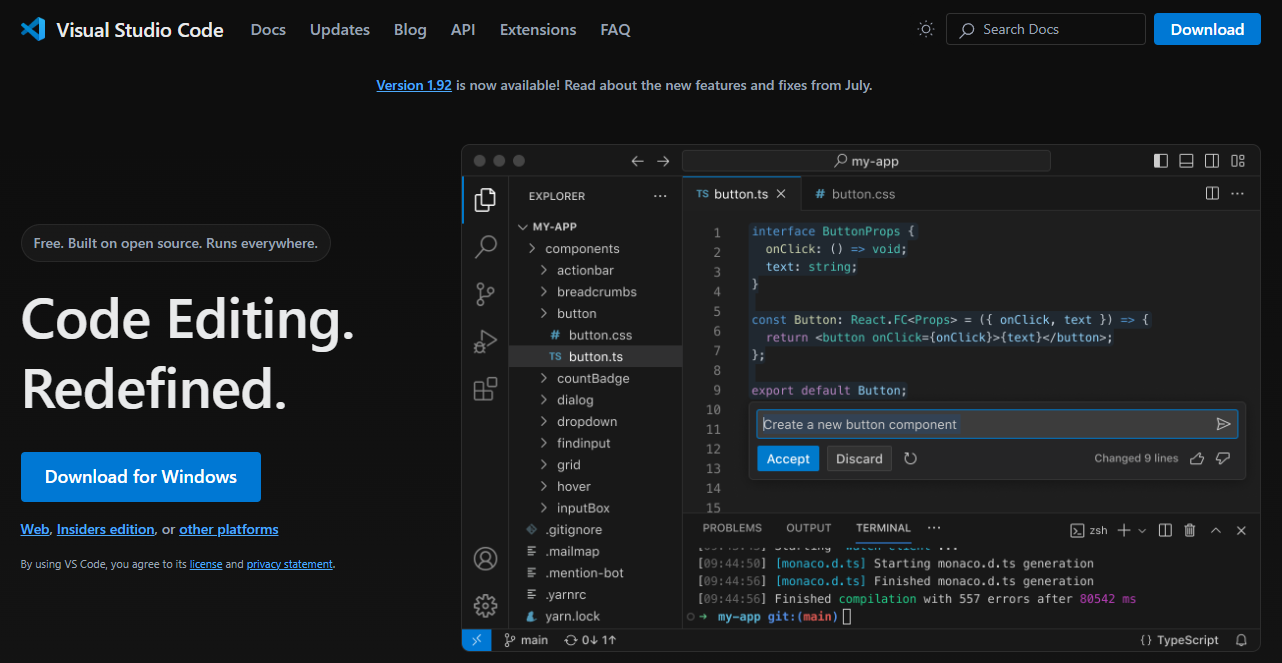
\includegraphics[width=0.8\textwidth]{figures/VSCodeWebsite.png}
              \caption{Visual Studio Code官网}
              \label{fig:VSCodeWebsite}
          \end{figure}
    \item 在Visual Studio Code中向本地安装扩展:WSL,以允许用户在Windows中使用Linux环境,如\cref{fig:ConfigureWSL}。
          \begin{figure}[htbp]
              \centering
              
\includegraphics[width=0.8\textwidth]{figures/ConfigureWSL.png}
              \caption{安装WSL扩展}
              \label{fig:ConfigureWSL}
          \end{figure}
    \item 在“控制面板”>“程序”>“程序和功能”>“启用或关闭Windows功能”中,确定“适用于Linux的Windows子系统”已被选中。
    \item 在“Windows任务管理器”>“性能”>“CPU”选项卡中,确定“虚拟化”已启用。
    \item 启动Windows PowerShell,执行命令\texttt{wsl --version},以查看WSL版本,命令执行结果如\cref{fig:WSLVersion},以验证安装成功。
          \begin{figure}[htbp]
              \centering
              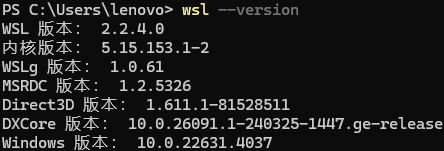
\includegraphics[width=0.6\textwidth]{figures/WSLVersion.png}
              \caption{WSL版本信息}
              \label{fig:WSLVersion}
          \end{figure}
\end{enumerate}

\subsubsection{配置Ubuntu 22.04 LTS}

Ubuntu 22.04 LTS可以为操作系统内核的开发提供一个稳定、高效、兼容性好的基础,同时也利于将来在类似环境中部署和运行。

下面是配置Ubuntu 22.04 LTS的步骤:

\begin{enumerate}
    \item 启动Windows PowerShell,执行命令\texttt{wsl --install Ubuntu-22.04},以安装Ubuntu 22.04 LTS版本到WSL,命令执行结果如\cref{fig:ConfigureUbuntu}。
          \begin{figure}[htbp]
              \centering
              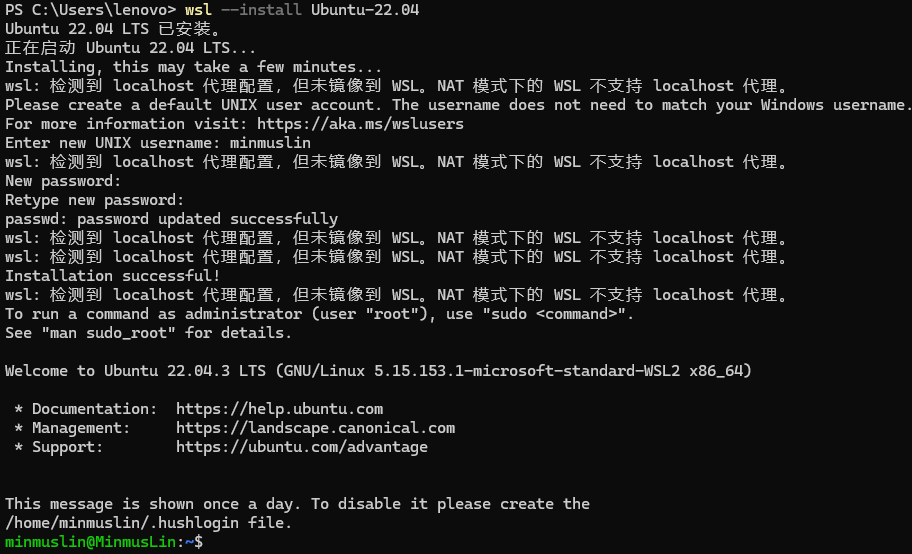
\includegraphics[width=0.8\textwidth]{figures/ConfigureUbuntu.png}
              \caption{配置Ubuntu 22.04 LTS}
              \label{fig:ConfigureUbuntu}
          \end{figure}
    \item 在Ubuntu中执行命令\texttt{lsb\_release -a},以查看Linux发行版的详细信息,命令执行结果如\cref{fig:UbuntuVersion},以验证安装成功。
          \begin{figure}[htbp]
              \centering
              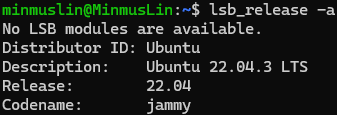
\includegraphics[width=0.5\textwidth]{figures/UbuntuVersion.png}
              \caption{Ubuntu版本信息}
              \label{fig:UbuntuVersion}
          \end{figure}
\end{enumerate}

\subsubsection{配置Rust语言开发环境}

Rust是一种注重安全、并发和性能的系统编程语言,旨在帮助开发者构建可靠和高效的软件。RustRover是JetBrains开发的针对于Rust编程语言的集成开发环境(IDE),对Rust语言开发提供了良好的支持。

配置Rust语言开发环境的步骤如下:

\begin{enumerate}
    \item 在JetBrains官网下载并安装JetBrains RustRover,如\cref{fig:RustRoverWebsite}。
          \begin{figure}[htbp]
              \centering
              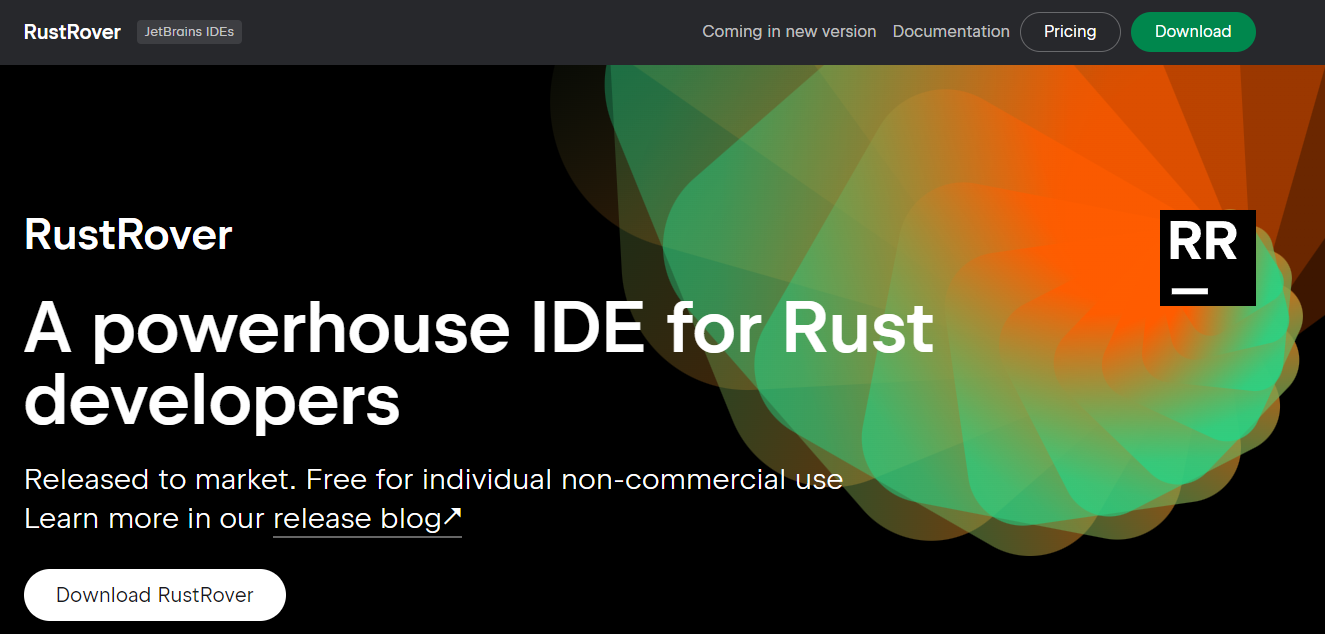
\includegraphics[width=0.8\textwidth]{figures/RustRoverWebsite.png}
              \caption{JetBrains官网}
              \label{fig:RustRoverWebsite}
          \end{figure}
    \item 启动RustRover,在“文件”>“远程开发”>“连接到WSL”中,选择WSL实例为“Ubuntu-22.04”,点击“下一页”。
    \item 在“选择IDE和项目”中,选择IDE版本为“RustRover 2024.1.7 (241.18034.106) | 下载最新”,选择项目目录为“/home/minmuslin/MinmusOS”,如\cref{fig:ConfigureRemoteDevelopment},点击“下载IDE并连接”。
          \begin{figure}[htbp]
              \centering
              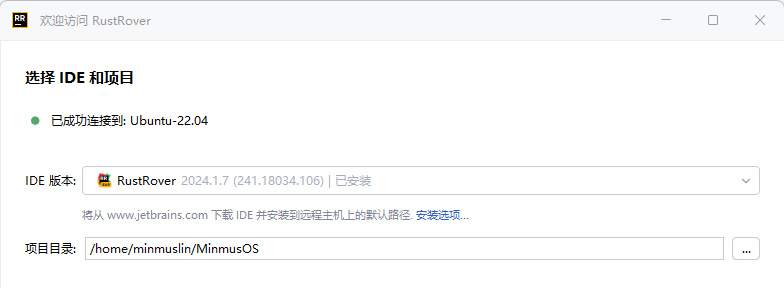
\includegraphics[width=0.8\textwidth]{figures/ConfigureRemoteDevelopment.png}
              \caption{配置远程开发}
              \label{fig:ConfigureRemoteDevelopment}
          \end{figure}
    \item 新建终端,执行\cref{lst:ConfigureRust},以配置Rust工具链,代码执行结果如\cref{fig:RustVersion},以验证安装成功。每行代码的作用如下:
          \begin{enumerate}
              \item \texttt{curl --proto '=https' --tlsv1.2 -sSf https://sh.rustup.rs | sh}:这行代码通过curl命令从指定的URL下载Rust安装脚本,并通过管道(|)将其传递给sh(Shell)来执行。选项--proto '=https'确保使用HTTPS协议,--tlsv1.2指定使用TLSv1.2版本进行安全连接,-sSf是几个选项的组合,-s表示静默模式,-S表示错误时显示错误,-f表示失败时不显示HTTP错误。
              \item \texttt{source \$HOME/.cargo/env}:执行这行代码会加载Rust的环境配置文件,该文件通常由rustup安装程序在安装Rust时创建于\$HOME/.cargo目录下。source命令用于执行该文件中的命令,以便在当前会话中设置环境变量,使得Rust工具链(如rustc、cargo)可以直接在命令行中使用。
              \item \texttt{rustup update}:这条命令用于更新Rust工具链到最新版本。rustup是Rust的版本管理和安装工具,可以用来管理不同的Rust版本和相关工具。
              \item \texttt{rustup default nightly}:设置Rust的默认工作版本为“nightly”版本。Rust有几个发布频道:stable、beta和nightly。nightly频道提供最新的功能,但可能不够稳定。这行命令将nightly频道设置为默认的Rust版本。
              \item \texttt{rustup --version}:显示当前安装的rustup工具的版本信息。这对于确认rustup是否成功安装及其版本非常有用。
              \item \texttt{rustup --version}:显示Rust编译器(rustc)的版本信息。这用于确认Rust编译器已经安装并可用,同时显示当前编译器的版本。
              \item \texttt{cargo --version}:显示Rust的包管理器和构建工具(cargo)的版本信息。Cargo用于Rust项目的依赖管理和构建,这行命令确认Cargo的安装状态及其版本。
          \end{enumerate}
          \begin{listing}[htbp]
              \begin{minted}{bash}
curl --proto '=https' --tlsv1.2 -sSf https://sh.rustup.rs | sh
source $HOME/.cargo/env
rustup update
rustup default nightly
rustup --version
rustc --version
cargo --version
              \end{minted}
              \caption{配置Rust工具链}\label{lst:ConfigureRust}
          \end{listing}
          \begin{figure}[htbp]
              \centering
              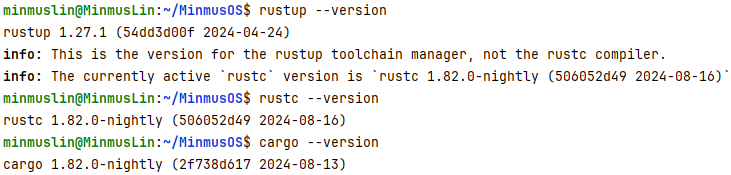
\includegraphics[width=0.8\textwidth]{figures/RustVersion.png}
              \caption{Rust版本信息}
              \label{fig:RustVersion}
          \end{figure}
\end{enumerate}

\subsubsection{配置编译环境与QEMU模拟机(qemu-system-i386)}

在Ubuntu系统配置编译环境的过程中,需要安装一系列的基本工具和库,以支持软件的编译和构建。执行命令\texttt{sudo apt update \&\& sudo apt install build-essential mtools dosfstools fdisk qemu-system-x86}以配置编译环境与QEMU模拟机(qemu-system-i386)。

每个安装的包的作用如下:

\begin{enumerate}
    \item \texttt{build-essential}:这是一个包含编译软件所需的基本编译工具(如gcc编译器、make工具等)的元包。
    \item \texttt{mtools}:一套用来访问MS-DOS磁盘和文件系统的工具,这在处理与DOS或Windows系统相关的磁盘映像时非常有用。
    \item \texttt{dosfstools}:包含用于创建和验证MS-DOS FAT文件系统在Unix和类Unix系统上的磁盘的工具,如mkfs.vfat工具。
    \item \texttt{fdisk}:一个磁盘分区表操作工具,用于创建和修改磁盘分区。
    \item \texttt{qemu-system-x86}:qemu-system-x86是QEMU(Quick Emulator)项目的一部分,它是一个功能强大的开源模拟器和虚拟化工具。特别地,qemu-system-x86是用于模拟x86和x86\_64(也称为AMD64)架构计算机的程序。这使得开发者和测试者可以在不同的操作系统和硬件配置上模拟和运行软件,而无需物理硬件。
\end{enumerate}

\subsection{运行MinmusOS项目}